\begin{figure}\centering\footnotesize
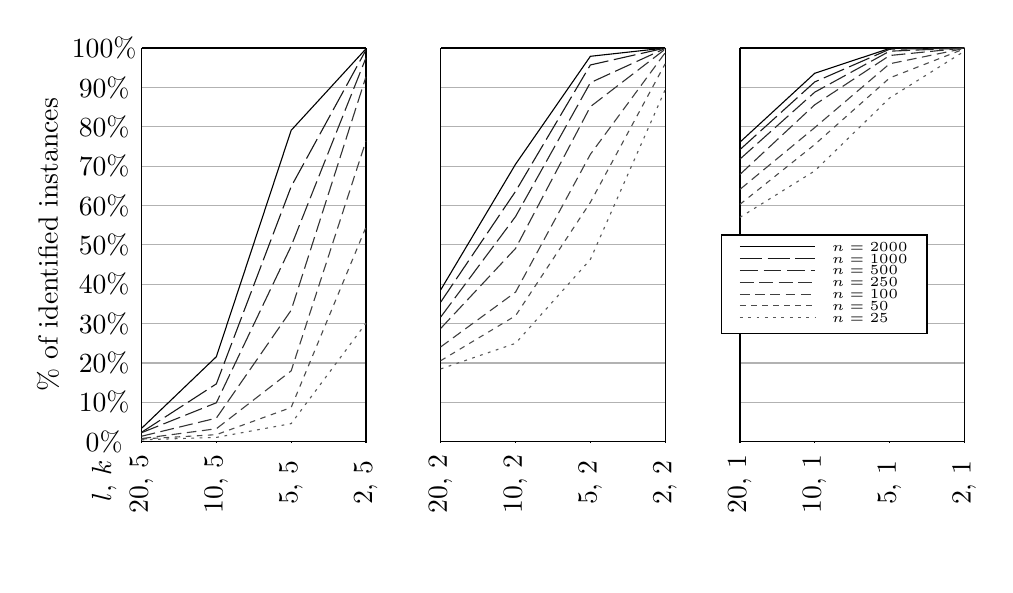
\begin{tikzpicture}[minimum size=0,xscale=0.95,yscale=0.5]
\node[] at (6, -1) {};
%\draw[] (0, 0) -- (12, 0);
%\draw (0, -0.03) -- (0, 0.03);
\node[rotate=90,text width=2.4cm] at (0.5, -.5) {\makebox[4mm]{\hfill}\phantom{,} \makebox[6mm]{\hfill$l$, $k$}};
\draw (1, -0.03) -- (1, 0.03);
\node[rotate=90,text width=2.4cm] at (1, -0.5) {\makebox[4mm]{\hfill}\phantom{,} \makebox[6mm]{\hfill$20$, $5$}};
\draw (2, -0.03) -- (2, 0.03);
\node[rotate=90,text width=2.4cm] at (2, -0.5) {\makebox[4mm]{\hfill}\phantom{,} \makebox[6mm]{\hfill$10$, $5$}};
\draw (3, -0.03) -- (3, 0.03);
\node[rotate=90,text width=2.4cm] at (3, -0.5) {\makebox[4mm]{\hfill}\phantom{,} \makebox[6mm]{\hfill$5$, $5$}};
\draw (4, -0.03) -- (4, 0.03);
\node[rotate=90,text width=2.4cm] at (4, -0.5) {\makebox[4mm]{\hfill}\phantom{,} \makebox[6mm]{\hfill$2$, $5$}};
\draw (5, -0.03) -- (5, 0.03);
\node[rotate=90,text width=2.4cm] at (5, -0.5) {\makebox[4mm]{\hfill}\phantom{,} \makebox[6mm]{\hfill$20$, $2$}};
\draw (6, -0.03) -- (6, 0.03);
\node[rotate=90,text width=2.4cm] at (6, -0.5) {\makebox[4mm]{\hfill}\phantom{,} \makebox[6mm]{\hfill$10$, $2$}};
\draw (7, -0.03) -- (7, 0.03);
\node[rotate=90,text width=2.4cm] at (7, -0.5) {\makebox[4mm]{\hfill}\phantom{,} \makebox[6mm]{\hfill$5$, $2$}};
\draw (8, -0.03) -- (8, 0.03);
\node[rotate=90,text width=2.4cm] at (8, -0.5) {\makebox[4mm]{\hfill}\phantom{,} \makebox[6mm]{\hfill$2$, $2$}};
\draw (9, -0.03) -- (9, 0.03);
\node[rotate=90,text width=2.4cm] at (9, -0.5) {\makebox[4mm]{\hfill}\phantom{,} \makebox[6mm]{\hfill$20$, $1$}};
\draw (10, -0.03) -- (10, 0.03);
\node[rotate=90,text width=2.4cm] at (10, -0.5) {\makebox[4mm]{\hfill}\phantom{,} \makebox[6mm]{\hfill$10$, $1$}};
\draw (11, -0.03) -- (11, 0.03);
\node[rotate=90,text width=2.4cm] at (11, -0.5) {\makebox[4mm]{\hfill}\phantom{,} \makebox[6mm]{\hfill$5$, $1$}};
\draw (12, -0.03) -- (12, 0.03);
\node[rotate=90,text width=2.4cm] at (12, -0.5) {\makebox[4mm]{\hfill}\phantom{,} \makebox[6mm]{\hfill$2$, $1$}};
\node[rotate=90] at (-0.25, 5) {\% of identified instances};
%\draw[] (0, 0) -- (0, 10);
%\draw (-0.03, 0) -- (0.03, 0);
\node[] at (0.5, 0) {0\%};
%\draw (-0.03, 1) -- (0.03, 1);
\node[] at (0.5, 1) {10\%};
%\draw (-0.03, 2) -- (0.03, 2);
\node[] at (0.5, 2) {20\%};
%\draw (-0.03, 3) -- (0.03, 3);
\node[] at (0.5, 3) {30\%};
%\draw (-0.03, 4) -- (0.03, 4);
\node[] at (0.5, 4) {40\%};
%\draw (-0.03, 5) -- (0.03, 5);
\node[] at (0.5, 5) {50\%};
%\draw (-0.03, 6) -- (0.03, 6);
\node[] at (0.5, 6) {60\%};
%\draw (-0.03, 7) -- (0.03, 7);
\node[] at (0.5, 7) {70\%};
%\draw (-0.03, 8) -- (0.03, 8);
\node[] at (0.5, 8) {80\%};
%\draw (-0.03, 9) -- (0.03, 9);
\node[] at (0.5, 9) {90\%};
%\draw (-0.03, 10) -- (0.03, 10);
\node[] at (0.5, 10) {100\%};
%\node[rotate=90] at (13.5, 5) {\% of identified instances};
\draw[] (12, 0) -- (12, 10);
%\draw (11.97, 0) -- (12.03, 0);
%\node[] at (12.75, 0) {0\%};
%\draw (11.97, 1) -- (12.03, 1);
%\node[] at (12.75, 1) {10\%};
%\draw (11.97, 2) -- (12.03, 2);
%\node[] at (12.75, 2) {20\%};
%\draw (11.97, 3) -- (12.03, 3);
%\node[] at (12.75, 3) {30\%};
%\draw (11.97, 4) -- (12.03, 4);
%\node[] at (12.75, 4) {40\%};
%\draw (11.97, 5) -- (12.03, 5);
%\node[] at (12.75, 5) {50\%};
%\draw (11.97, 6) -- (12.03, 6);
%\node[] at (12.75, 6) {60\%};
%\draw (11.97, 7) -- (12.03, 7);
%\node[] at (12.75, 7) {70\%};
%\draw (11.97, 8) -- (12.03, 8);
%\node[] at (12.75, 8) {80\%};
%\draw (11.97, 9) -- (12.03, 9);
%\node[] at (12.75, 9) {90\%};
%\draw (11.97, 10) -- (12.03, 10);
%\node[] at (12.75, 10) {100\%};
\draw[        ] (1, 0) -- ( 4, 0) (5, 0) -- ( 8, 0) (9, 0) -- (12, 0);
\draw[black!30] (1, 1) -- ( 4, 1) (5, 1) -- ( 8, 1) (9, 1) -- (12, 1);
\draw[black!30] (1, 2) -- ( 4, 2) (5, 2) -- ( 8, 2) (9, 2) -- (12, 2);
\draw[black!30] (1, 3) -- ( 4, 3) (5, 3) -- ( 8, 3) (9, 3) -- (12, 3);
\draw[black!30] (1, 4) -- ( 4, 4) (5, 4) -- ( 8, 4) (9, 4) -- (12, 4);
\draw[black!30] (1, 5) -- ( 4, 5) (5, 5) -- ( 8, 5) (9, 5) -- (12, 5);
\draw[black!30] (1, 6) -- ( 4, 6) (5, 6) -- ( 8, 6) (9, 6) -- (12, 6);
\draw[black!30] (1, 7) -- ( 4, 7) (5, 7) -- ( 8, 7) (9, 7) -- (12, 7);
\draw[black!30] (1, 8) -- ( 4, 8) (5, 8) -- ( 8, 8) (9, 8) -- (12, 8);
\draw[black!30] (1, 9) -- ( 4, 9) (5, 9) -- ( 8, 9) (9, 9) -- (12, 9);
\draw[        ] (1,10) -- ( 4,10) (5,10) -- ( 8,10) (9,10) -- (12,10);
\draw[] (1, 0) -- (1, 10);
\draw[] (4, 0) -- (4, 10);
\draw[] (5, 0) -- (5, 10);
\draw[] (8, 0) -- (8, 10);
\draw[] (9, 0) -- (9, 10);
\draw[black] (1, 0.34) -- (2, 2.16) -- (3, 7.91) -- (4, 9.98)  
            (5, 3.86) -- (6, 7.05) -- (7, 9.79) -- (8, 10) 
            (9, 7.61) -- (10, 9.36) -- (11, 9.99) -- (12, 10); 
\draw[white!10!black, dash pattern={on 8pt off 2pt}] 
            (1, 0.24) -- (2, 1.47) -- (3, 6.48) -- (4, 9.95)  
            (5, 3.55) -- (6, 6.36) -- (7, 9.57) -- (8, 10) 
            (9, 7.42) -- (10, 9.14) -- (11, 9.97) -- (12, 10); 
\draw[white!15!black, dash pattern={on 6.5pt off 2pt}] 
            (1, 0.23) -- (2, 0.99) -- (3, 4.97) -- (4, 9.75) 
            (5, 3.17) -- (6, 5.72) -- (7, 9.12) -- (8, 9.99) 
            (9, 7.18) -- (10, 8.88) -- (11, 9.92) -- (12, 10); 
\draw[white!20!black, dash pattern={on 5pt off 2pt}] 
            (1, 0.14) -- (2, 0.6) -- (3, 3.34) -- (4, 9.27) 
            (5, 2.88) -- (6, 4.91) -- (7, 8.51) -- (8, 9.97)
            (9, 6.79) -- (10, 8.56) -- (11, 9.81) -- (12, 10); 
\draw[white!25!black, dash pattern={on 3.5pt off 2pt}] 
            (1, 0.08) -- (2, 0.33) -- (3, 1.8) -- (4, 7.64) 
            (5, 2.41) -- (6, 3.8) -- (7, 7.3) -- (8, 9.88) 
            (9, 6.41) -- (10, 7.98) -- (11, 9.6) -- (12, 9.99); 
%\draw[white!30!red, dash pattern={on 2pt off 2pt}]           old results
%            (1, 0.05) -- (2, 0.17) -- (3, 0.89) -- (4, 5.46) 
%            (5, 2.25) -- (6, 3.3) -- (7, 5.82) -- (8, 9.52) 
%            (9, 6.03) -- (10, 7.55) -- (11, 9.24) -- (12, 9.98); 
\draw[white!30!black, dash pattern={on 2pt off 2pt}] 
            (1, 0.07) -- (2, 0.18) -- (3, 0.87) -- (4, 5.45) 
            (5, 2.06) -- (6, 3.2) -- (7, 6.08) -- (8, 9.6) 
            (9, 6.03) -- (10, 7.55) -- (11, 9.24) -- (12, 9.98); 
\draw[white!35!black, dash pattern={on 1pt off 2pt}] (1, 0.05) -- (2, 0.11) -- (3, 0.46) -- (4, 3.01) 
              (5, 1.85) -- (6, 2.5) -- (7, 4.63) -- (8, 8.94) 
              (9, 5.7) -- (10, 6.88) -- (11, 8.73) -- (12, 9.92); 
%\node[draw,black!60!orange,cross out] at (1, 0.25) {};
%\node[draw,black!60!orange,cross out] at (2, 1.32) {};
%\node[draw,black!60!orange,cross out] at (3, 6.76) {};
%\node[draw,black!60!orange,cross out] at (4, 9.96) {};
%\node[draw,black!60!orange,cross out] at (5, 3.44) {};
%\node[draw,black!60!orange,cross out] at (6, 6.07) {};
%\node[draw,black!60!orange,cross out] at (7, 9.36) {};
%\node[draw,black!60!orange,cross out] at (8, 9.99) {};
%\node[draw,black!60!orange,cross out] at (9, 6.8) {};
%\node[draw,black!60!orange,cross out] at (10, 8.58) {};
%\node[draw,black!60!orange,cross out] at (11, 9.83) {};
%\node[draw,black!60!orange,cross out] at (12, 10) {};
%\node[draw,black!40!orange,cross out] at (1, 0.16) {};
%\node[draw,black!40!orange,cross out] at (2, 0.8) {};
%\node[draw,black!40!orange,cross out] at (3, 4.69) {};
%\node[draw,black!40!orange,cross out] at (4, 9.8) {};
%\node[draw,black!40!orange,cross out] at (5, 2.94) {};
%\node[draw,black!40!orange,cross out] at (6, 4.99) {};
%\node[draw,black!40!orange,cross out] at (7, 8.62) {};
%\node[draw,black!40!orange,cross out] at (8, 9.98) {};
%\node[draw,black!40!orange,cross out] at (9, 6.42) {};
%\node[draw,black!40!orange,cross out] at (10, 7.99) {};
%\node[draw,black!40!orange,cross out] at (11, 9.62) {};
%\node[draw,black!40!orange,cross out] at (12, 9.99) {};
%\node[draw,black!20!orange,cross out] at (1, 0.1) {};
%\node[draw,black!20!orange,cross out] at (2, 0.5) {};
%\node[draw,black!20!orange,cross out] at (3, 3.08) {};
%\node[draw,black!20!orange,cross out] at (4, 9.4) {};
%\node[draw,black!20!orange,cross out] at (5, 2.59) {};
%\node[draw,black!20!orange,cross out] at (6, 4.1) {};
%\node[draw,black!20!orange,cross out] at (7, 7.31) {};
%\node[draw,black!20!orange,cross out] at (8, 9.89) {};
%\node[draw,black!20!orange,cross out] at (9, 6.03) {};
%\node[draw,black!20!orange,cross out] at (10, 7.56) {};
%\node[draw,black!20!orange,cross out] at (11, 9.25) {};
%\node[draw,black!20!orange,cross out] at (12, 9.98) {};
%\node[draw,orange,cross out] at (1, 0.07) {};
%\node[draw,orange,cross out] at (2, 0.25) {};
%\node[draw,orange,cross out] at (3, 1.46) {};
%\node[draw,orange,cross out] at (4, 8.16) {};
%\node[draw,orange,cross out] at (5, 2.07) {};
%\node[draw,orange,cross out] at (6, 3.37) {};
%\node[draw,orange,cross out] at (7, 6.16) {};
%\node[draw,orange,cross out] at (8, 9.63) {};
%\node[draw,orange,cross out] at (9, 5.7) {};
%\node[draw,orange,cross out] at (10, 6.89) {};
%\node[draw,orange,cross out] at (11, 8.74) {};
%\node[draw,orange,cross out] at (12, 9.93) {};
\draw[draw=black,fill=white] (8.75, 5.25) rectangle (11.5, 2.75);
\draw[black] (9, 4.95) -- (10, 4.95); 
\node[anchor=west] at (10.1, 4.95) {\tiny $n = 2000$};
\draw[white!10!black, dash pattern={on 8pt off 2pt}] (9, 4.65) -- (10, 4.65); 
\node[anchor=west] at (10.1, 4.65) {\tiny $n = 1000$};
\draw[white!15!black, dash pattern={on 6.5pt off 2pt}] (9, 4.35) -- (10, 4.35); 
\node[anchor=west] at (10.1, 4.35) {\tiny $n = 500$};
\draw[white!20!black, dash pattern={on 5pt off 2pt}] (9, 4.05) -- (10, 4.05); 
\node[anchor=west] at (10.1, 4.05) {\tiny $n = 250$};
\draw[white!25!black, dash pattern={on 3.5pt off 2pt}] (9, 3.75) -- (10, 3.75); 
\node[anchor=west] at (10.1, 3.75) {\tiny $n = 100$};
\draw[white!30!black, dash pattern={on 2pt off 2pt}] (9, 3.45) -- (10, 3.45); 
\node[anchor=west] at (10.1, 3.45) {\tiny $n = 50$};
\draw[white!35!black, dash pattern={on 1pt off 2pt}] (9, 3.15) -- (10, 3.15); 
\node[anchor=west] at (10.1, 3.15) {\tiny $n = 25$};
%(9, 2.85) -- (10, 2.85); 
%\node[draw,black!60!orange,cross out] at (9.5, 2.85) {};
%\node[anchor=west] at (10.1, 2.85) {$n = 250$};
%(9, 2.55) -- (10, 2.55); 
%\node[draw,black!40!orange,cross out] at (9.5, 2.55) {};
%\node[anchor=west] at (10.1, 2.55) {$n = 100$};
%(9, 2.25) -- (10, 2.25); 
%\node[draw,black!20!orange,cross out] at (9.5, 2.25) {};
%\node[anchor=west] at (10.1, 2.25) {$n = 50$};
%(9, 1.95) -- (10, 1.95); 
%\node[draw,orange,cross out] at (9.5, 1.95) {};
%\node[anchor=west] at (10.1, 1.95) {$n = 25$};
\end{tikzpicture}
\caption{Case $P(\textit{unobserved}=0.75)$:
Percent of identifiable graphs for fixed numbers of nodes $n\in\{25,50,100,250,500,1000,2000\}$ and
with varying  expected number of node neighbors  $l$ and cardinalities 
$|\bX|=|\bY|=k$. The horizontal axis is labeled by $(l,k)$ sorted lexicographically.
The curves show the data for CBC$^+$, i.e., for instances identifiable by adjustment 
or by plain formula. 
%; The crosses represent the data for IDC, i.e. for cases that 
%are identifiable at all. The high time complexity of the IDC algorithm precluded computations
%for graphs of sizes  $n\ge 500$.
}\label{fig:global:n:curves}
\end{figure}
